\chapter{Diagrama de Casos de Uso}\label{cap:4-diag-casos}

A partir dos requisitos funcionais descritos no capítulo \ref{cap:3-reqs-f-e-nf}, foi elaborado o diagrama da figura \ref{fig:diag-casos-uso} de casos de uso do sistema. Este diagrama ilustra as interações entre o usuário e o sistema, destacando as principais funcionalidades que serão implementadas.

\begin{figure}[h]
    \centering
    \caption{Diagrama de casos de uso.}
    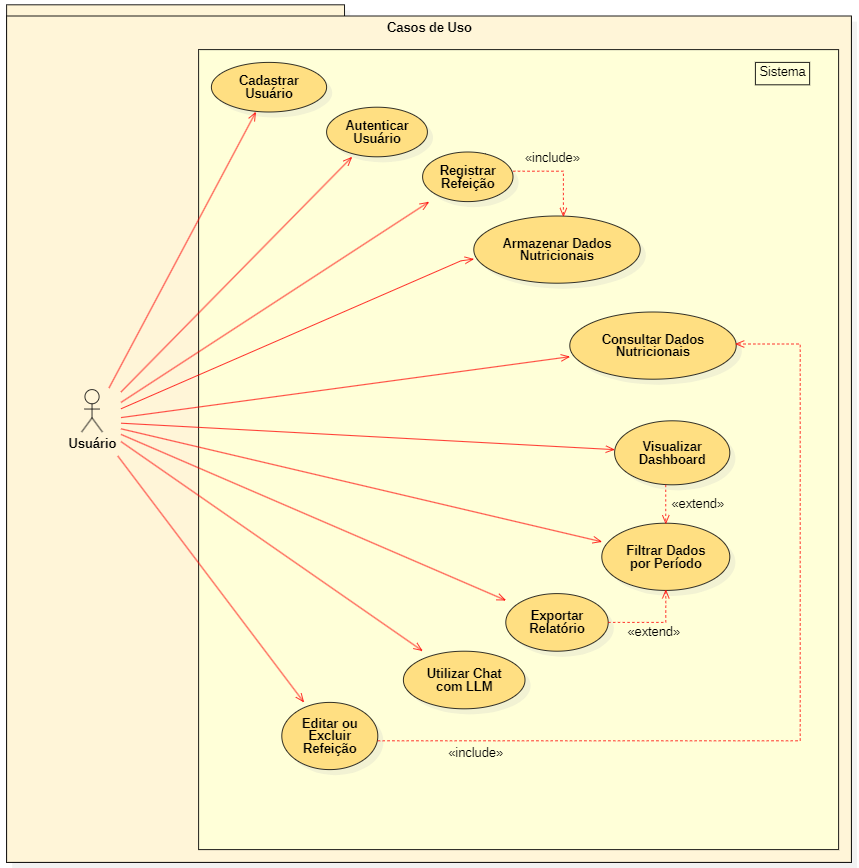
\includegraphics[width=0.92\textwidth]{Figuras/diagrama-casos-uso.png}\\
    \small{\textbf{Fonte}: Autor (2025).}
    \label{fig:diag-casos-uso}
\end{figure}

Na tabela \ref{tab:casos-de-uso} a seguir, estão listados os casos de uso identificados, juntamente com o seu nome. Cada caso de uso representa uma funcionalidade específica do sistema e está associado a um código único para facilitar a referência.

\begin{longtable}[c]{|l|l|}
\caption{Casos de uso e seus códigos.}
\label{tab:casos-de-uso}\\
\hline
\textbf{Código} & \textbf{Descrição}           \\ \hline
\endfirsthead
\endhead
UC01            & Cadastrar Usuário            \\ \hline
UC02            & Autenticar Usuário           \\ \hline
UC03            & Registrar Refeição           \\ \hline
UC04            & Armazenar Dados Nutricionais \\ \hline
UC05            & Consultar Dados Nutricionais \\ \hline
UC06            & Visualizar Dashboard         \\ \hline
UC07            & Filtrar Dados do Período     \\ \hline
UC08            & Exportar Relatório           \\ \hline
UC09            & Utilizar Chat com LLM        \\ \hline
UC10            & Editar ou Excluir Refeição   \\ \hline
\end{longtable}
\begin{center}
    \small{\textbf{Fonte}: Autor (2025).}
\end{center}

Com os casos de uso definidos, o próximo passo é fazer a sua associação com os requisitos funcionais, garantindo que todas as funcionalidades do sistema estejam contempladas. A tabela \ref{tab:casos-uso-requisitos-funcionais} a seguir apresenta essa associação, indicando quais casos de uso atendem a cada requisito funcional.

\begin{table}[h]
    \centering
    \caption{Casos de uso e sua associação com os Requisistos Funcionais.}
    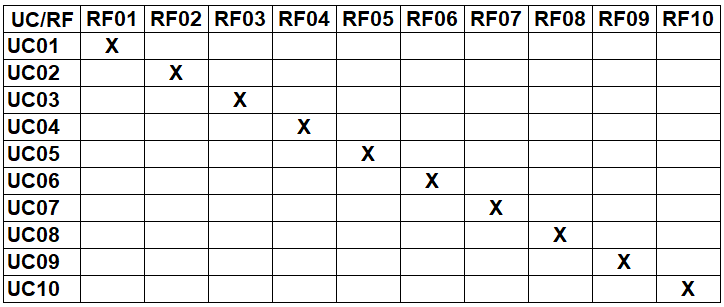
\includegraphics[width=0.92\textwidth]{Tabelas/casos-uso-relacao-reqs-func.png}\\
    \small{\textbf{Fonte}: Autor (2025).}
    \label{tab:casos-uso-requisitos-funcionais}
\end{table}


\section{Definição completa dos Casos de Uso}

A seguir, são apresentados os casos de uso detalhados, com suas descrições, pré-condições, pós-condições e fluxos de eventos. Esses detalhes são essenciais para compreender como cada funcionalidade será implementada e como o usuário interagirá com o sistema.

% UC01 - Cadastrar Usuário
\subsection{UC01 - Cadastrar Usuário}

\begin{longtable}[c]{|p{0.48\textwidth}|p{0.48\textwidth}|}
\caption{UC01: Cadastrar Usuário}
\label{tab:uc01}\\
\hline
\multicolumn{1}{|p{0.48\textwidth}|}{\textbf{Nome}} &
  \begin{tabular}[c]{@{}p{0.48\textwidth}@{}}UC01: Cadastrar Usuário\end{tabular} \\ \hline
\endfirsthead
%
\endhead
%
\multicolumn{1}{|p{0.48\textwidth}|}{\textbf{Atores}} &
  \begin{tabular}[c]{@{}p{0.48\textwidth}@{}}Usuário\end{tabular} \\ \hline
\multicolumn{1}{|p{0.48\textwidth}|}{\textbf{Descrição}} &
  \begin{tabular}[c]{@{}p{0.48\textwidth}@{}}Permite que um novo usuário crie uma conta no sistema informando os dados obrigatórios, garantindo a unicidade do login e a segurança das informações.\end{tabular} \\ \hline
\multicolumn{1}{|p{0.48\textwidth}|}{\textbf{Pré-condições}} &
  \begin{tabular}[c]{@{}p{0.48\textwidth}@{}}O usuário deve ter acessado a aplicação; O usuário não pode estar autenticado; Não deve existir outra conta com o mesmo login.\end{tabular} \\ \hline
\multicolumn{1}{|p{0.48\textwidth}|}{\textbf{Pós-condições}} &
  \begin{tabular}[c]{@{}p{0.48\textwidth}@{}}Conta do usuário criada, pronta para autenticar.\end{tabular} \\ \hline
\multicolumn{2}{|c|}{\textbf{Fluxo Básico}} \\ \hline
\multicolumn{1}{|c|}{\textbf{Ações do Ator}} &
  \multicolumn{1}{c|}{\textbf{Ações do Sistema}} \\ \hline
\multicolumn{1}{|p{0.48\textwidth}|}{\begin{tabular}[c]{@{}p{0.48\textwidth}@{}}1. Acessa a tela de cadastro pelo menu inicial ou por link de criar conta.\end{tabular}} &
   \\ \hline
\multicolumn{1}{|p{0.48\textwidth}|}{} &
  \begin{tabular}[c]{@{}p{0.48\textwidth}@{}}2. Exibe formulário de cadastro com campos obrigatórios (login/e-mail; senha; confirmação da senha; data de nascimento; aceite dos termos).\end{tabular} \\ \hline
\multicolumn{1}{|p{0.48\textwidth}|}{\begin{tabular}[c]{@{}p{0.48\textwidth}@{}}3. Preenche as informações de forma adequada.\end{tabular}} &
   \\ \hline
\multicolumn{1}{|p{0.48\textwidth}|}{\begin{tabular}[c]{@{}p{0.48\textwidth}@{}}4. Clica no botão ``Cadastrar" para submeter as informações digitadas.\end{tabular}} &
   \\ \hline
\multicolumn{1}{|p{0.48\textwidth}|}{} &
  \begin{tabular}[c]{@{}p{0.48\textwidth}@{}}5. Valida se todos os campos obrigatórios foram preenchidos (RN01, RN02, RN08, RN10).\end{tabular} \\ \hline
\multicolumn{1}{|p{0.48\textwidth}|}{} &
  \begin{tabular}[c]{@{}p{0.48\textwidth}@{}}6. Valida o formato do e-mail (RN04).\end{tabular} \\ \hline
\multicolumn{1}{|p{0.48\textwidth}|}{} &
  \begin{tabular}[c]{@{}p{0.48\textwidth}@{}}7. Valida a força da senha (RN05, RN06).\end{tabular} \\ \hline
\multicolumn{1}{|p{0.48\textwidth}|}{} &
  \begin{tabular}[c]{@{}p{0.48\textwidth}@{}}8. Verifica se o login já está cadastrado (RN03).\end{tabular} \\ \hline
\multicolumn{1}{|p{0.48\textwidth}|}{} &
  \begin{tabular}[c]{@{}p{0.48\textwidth}@{}}9. Valida a idade do usuário (RN08).\end{tabular} \\ \hline
\multicolumn{1}{|p{0.48\textwidth}|}{} &
  \begin{tabular}[c]{@{}p{0.48\textwidth}@{}}10. Valida a aceitação dos termos (RN10).\end{tabular} \\ \hline
\multicolumn{1}{|p{0.48\textwidth}|}{} &
  \begin{tabular}[c]{@{}p{0.48\textwidth}@{}}11. Ao aprovar todas as validações, armazena os dados do usuário, criptografa a senha (RN07) e registra a data e hora do cadastro (RN11).\end{tabular} \\ \hline
\multicolumn{1}{|p{0.48\textwidth}|}{} &
  \begin{tabular}[c]{@{}p{0.48\textwidth}@{}}12. Exibe a mensagem de sucesso ``Usuário cadastrado com sucesso!"\end{tabular} \\ \hline
\multicolumn{1}{|p{0.48\textwidth}|}{} &
  \begin{tabular}[c]{@{}p{0.48\textwidth}@{}}13. Redireciona o usuário para a página de login.\end{tabular} \\ \hline
\multicolumn{2}{|c|}{\textbf{Regras de Negócio}} \\ \hline
\multicolumn{1}{|p{0.48\textwidth}|}{RN01} &
  \begin{tabular}[c]{@{}p{0.48\textwidth}@{}}O campo login (e-mail) é obrigatório.\end{tabular} \\ \hline
\multicolumn{1}{|p{0.48\textwidth}|}{RN02} &
  \begin{tabular}[c]{@{}p{0.48\textwidth}@{}}O campo de senha é obrigatório.\end{tabular} \\ \hline
\multicolumn{1}{|p{0.48\textwidth}|}{RN03} &
  \begin{tabular}[c]{@{}p{0.48\textwidth}@{}}O login deve ser único no sistema.\end{tabular} \\ \hline
\multicolumn{1}{|p{0.48\textwidth}|}{RN04} &
  \begin{tabular}[c]{@{}p{0.48\textwidth}@{}}O email deve estar em formato válido.\end{tabular} \\ \hline
\multicolumn{1}{|p{0.48\textwidth}|}{RN05} &
  \begin{tabular}[c]{@{}p{0.48\textwidth}@{}}A senha deve ter no mínimo 8 caracteres.\end{tabular} \\ \hline
\multicolumn{1}{|p{0.48\textwidth}|}{RN06} &
  \begin{tabular}[c]{@{}p{0.48\textwidth}@{}}A senha deve conter pelo menos uma letra maiúscula, uma minúscula, um número e um caractere especial.\end{tabular} \\ \hline
\multicolumn{1}{|p{0.48\textwidth}|}{RN07} &
  \begin{tabular}[c]{@{}p{0.48\textwidth}@{}}O sistema deve armazenar a senha de forma criptografada.\end{tabular} \\ \hline
\multicolumn{1}{|p{0.48\textwidth}|}{RN08} &
  \begin{tabular}[c]{@{}p{0.48\textwidth}@{}}O cadastro só é permitido para maiores de 18 anos.\end{tabular} \\ \hline
\multicolumn{1}{|p{0.48\textwidth}|}{RN09} &
  \begin{tabular}[c]{@{}p{0.48\textwidth}@{}}O sistema deve validar a regra de negócio RNF02 (autenticação via JWT).\end{tabular} \\ \hline
\multicolumn{1}{|p{0.48\textwidth}|}{RN10} &
  \begin{tabular}[c]{@{}p{0.48\textwidth}@{}}O usuário deve aceitar os termos de uso e política de privacidade.\end{tabular} \\ \hline
\multicolumn{1}{|p{0.48\textwidth}|}{RN11} &
  \begin{tabular}[c]{@{}p{0.48\textwidth}@{}}O sistema deve registrar a data e hora do cadastro.\end{tabular} \\ \hline
\multicolumn{2}{|c|}{\textbf{Fluxo Alternativo A: login já cadastrado}} \\ \hline
\multicolumn{1}{|c|}{\textbf{Ações do Ator}} &
  \multicolumn{1}{c|}{\textbf{Ações do Sistema}} \\ \hline
\multicolumn{1}{|p{0.48\textwidth}|}{\begin{tabular}[c]{@{}p{0.48\textwidth}@{}}1. Preenche o formulário com um e-mail já existente clica em ``Cadastrar".\end{tabular}} &
   \\ \hline
\multicolumn{1}{|p{0.48\textwidth}|}{} &
  \begin{tabular}[c]{@{}p{0.48\textwidth}@{}}2. Valida unicidade do login e identifica duplicidade.\end{tabular} \\ \hline
\multicolumn{1}{|p{0.48\textwidth}|}{} &
  \begin{tabular}[c]{@{}p{0.48\textwidth}@{}}3. Exibe mensagem de erro ``E-mail já cadastrado. Tente outro e-mail."\end{tabular} \\ \hline
\multicolumn{2}{|c|}{\textbf{Fluxo Alternativo B: senha fraca ou inválida}} \\ \hline
\multicolumn{1}{|c|}{\textbf{Ações do Ator}} &
  \multicolumn{1}{c|}{\textbf{Ações do Sistema}} \\ \hline
\multicolumn{1}{|p{0.48\textwidth}|}{\begin{tabular}[c]{@{}p{0.48\textwidth}@{}}1. Preenche o campo de senha com valor que não atende aos critérios e clica em ``Cadastrar".\end{tabular}} &
   \\ \hline
\multicolumn{1}{|p{0.48\textwidth}|}{} &
  \begin{tabular}[c]{@{}p{0.48\textwidth}@{}}2. Valida a força da senha e identifica não conformidade.\end{tabular} \\ \hline
\multicolumn{1}{|p{0.48\textwidth}|}{} &
  \begin{tabular}[c]{@{}p{0.48\textwidth}@{}}3. Exibe mensagem de erro detalhando os requisitos mínimos da senha\end{tabular} \\ \hline
\multicolumn{2}{|c|}{\textbf{Fluxo Alternativo C: campos obrigatórios não preenchidos}} \\ \hline
\multicolumn{1}{|c|}{\textbf{Ações do Ator}} &
  \multicolumn{1}{c|}{\textbf{Ações do Sistema}} \\ \hline
\multicolumn{1}{|p{0.48\textwidth}|}{\begin{tabular}[c]{@{}p{0.48\textwidth}@{}}1. Deixa um ou mais campos obrigatórios em branco e clica em ``Cadastrar".\end{tabular}} &
   \\ \hline
\multicolumn{1}{|p{0.48\textwidth}|}{} &
  \begin{tabular}[c]{@{}p{0.48\textwidth}@{}}2. Valida preenchimento dos campos e identifica ausência.\end{tabular} \\ \hline
\multicolumn{1}{|p{0.48\textwidth}|}{} &
  \begin{tabular}[c]{@{}p{0.48\textwidth}@{}}3. Exibe mensagem de erro informando quais campos precisam ser preenchidos.\end{tabular} \\ \hline
\multicolumn{2}{|c|}{\textbf{Fluxo Alternativo D: usuário menor de 18 anos}} \\ \hline
\multicolumn{1}{|c|}{\textbf{Ações do Ator}} &
  \multicolumn{1}{c|}{\textbf{Ações do Sistema}} \\ \hline
\multicolumn{1}{|p{0.48\textwidth}|}{\begin{tabular}[c]{@{}p{0.48\textwidth}@{}}1. Informa data de nascimento que indica idade inferior a 18 anos e clica em “Cadastrar”.\end{tabular}} &
   \\ \hline
\multicolumn{1}{|p{0.48\textwidth}|}{} &
  \begin{tabular}[c]{@{}p{0.48\textwidth}@{}}2. Valida idade e identifica restrição.\end{tabular} \\ \hline
\multicolumn{1}{|p{0.48\textwidth}|}{} &
  \begin{tabular}[c]{@{}p{0.48\textwidth}@{}}3. Exibe mensagem de erro ``Cadastro permitido apenas para maiores de 18 anos."\end{tabular} \\ \hline
\multicolumn{2}{|c|}{\textbf{Fluxo Alternativo E: e-mail em formato inválido}} \\ \hline
\multicolumn{1}{|c|}{\textbf{Ações do Ator}} &
  \multicolumn{1}{c|}{\textbf{Ações do Sistema}} \\ \hline
\multicolumn{1}{|p{0.48\textwidth}|}{\begin{tabular}[c]{@{}p{0.48\textwidth}@{}}1. Preenche o campo de e-mail com formato incorreto e clica em ``Cadastrar".\end{tabular}} &
   \\ \hline
\multicolumn{1}{|p{0.48\textwidth}|}{} &
  \begin{tabular}[c]{@{}p{0.48\textwidth}@{}}2. Valida formato do e-mail e identifica erro.\end{tabular} \\ \hline
\multicolumn{1}{|p{0.48\textwidth}|}{} &
  \begin{tabular}[c]{@{}p{0.48\textwidth}@{}}3. Exibe mensagem de erro ``E-mail em formato inválido."\end{tabular} \\ \hline
\multicolumn{2}{|c|}{\textbf{Fluxo Alternativo F: recarregamento da página}} \\ \hline
\multicolumn{1}{|c|}{\textbf{Ações do Ator}} &
  \multicolumn{1}{c|}{\textbf{Ações do Sistema}} \\ \hline
\multicolumn{1}{|p{0.48\textwidth}|}{\begin{tabular}[c]{@{}p{0.48\textwidth}@{}}1. Durante o preenchimento do formulário, recarrega a página do navegador.\end{tabular}} &
   \\ \hline
\multicolumn{1}{|p{0.48\textwidth}|}{} &
  \begin{tabular}[c]{@{}p{0.48\textwidth}@{}}2. Recarrega a tela de cadastro, perdendo todos os dados não salvos.\end{tabular} \\ \hline
\end{longtable}

% UC02 - Autenticar Usuário
\subsection{UC02 - Autenticar Usuário}

\begin{longtable}[c]{|p{0.48\textwidth}|p{0.48\textwidth}|}
\caption{UC02: Autenticar Usuário}
\label{tab:uc02}\\
\hline
\multicolumn{1}{|p{0.48\textwidth}|}{\textbf{Nome}} &
  \begin{tabular}[c]{@{}p{0.48\textwidth}@{}}UC02: Autenticar Usuário\end{tabular} \\ \hline
\endfirsthead
%
\endhead
%
\multicolumn{1}{|p{0.48\textwidth}|}{\textbf{Atores}} &
  \begin{tabular}[c]{@{}p{0.48\textwidth}@{}}Usuário\end{tabular} \\ \hline
\multicolumn{1}{|p{0.48\textwidth}|}{\textbf{Descrição}} &
  \begin{tabular}[c]{@{}p{0.48\textwidth}@{}}Permite que um usuário cadastrado acesse o sistema informando suas credenciais válidas, garantindo a segurança e a privacidade das informações.\end{tabular} \\ \hline
\multicolumn{1}{|p{0.48\textwidth}|}{\textbf{Pré-condições}} &
  \begin{tabular}[c]{@{}p{0.48\textwidth}@{}}O usuário deve ter cadastro prévio no sistema; O usuário não pode estar autenticado.\end{tabular} \\ \hline
\multicolumn{1}{|p{0.48\textwidth}|}{\textbf{Pós-condições}} &
  \begin{tabular}[c]{@{}p{0.48\textwidth}@{}}Usuário autenticado, sessão iniciada.\end{tabular} \\ \hline
\multicolumn{2}{|c|}{\textbf{Fluxo Básico}} \\ \hline
\multicolumn{1}{|c|}{\textbf{Ações do Ator}} &
  \multicolumn{1}{c|}{\textbf{Ações do Sistema}} \\ \hline
\multicolumn{1}{|p{0.48\textwidth}|}{\begin{tabular}[c]{@{}p{0.48\textwidth}@{}}1. Acessa a tela de login pelo menu inicial.\end{tabular}} &
   \\ \hline
\multicolumn{1}{|p{0.48\textwidth}|}{} &
  \begin{tabular}[c]{@{}p{0.48\textwidth}@{}}2. Exibe formulário de autenticação com campos obrigatórios (login/e-mail e senha).\end{tabular} \\ \hline
\multicolumn{1}{|p{0.48\textwidth}|}{\begin{tabular}[c]{@{}p{0.48\textwidth}@{}}3. Preenche o campo de e-mail e senha.\end{tabular}} &
   \\ \hline
\multicolumn{1}{|p{0.48\textwidth}|}{\begin{tabular}[c]{@{}p{0.48\textwidth}@{}}4. Clica no botão ``Entrar'' para submeter as informações.\end{tabular}} &
   \\ \hline
\multicolumn{1}{|p{0.48\textwidth}|}{} &
  \begin{tabular}[c]{@{}p{0.48\textwidth}@{}}5. Valida se os campos obrigatórios foram preenchidos (RN01, RN02).\end{tabular} \\ \hline
\multicolumn{1}{|p{0.48\textwidth}|}{} &
  \begin{tabular}[c]{@{}p{0.48\textwidth}@{}}6. Valida o formato do e-mail (RN04).\end{tabular} \\ \hline
\multicolumn{1}{|p{0.48\textwidth}|}{} &
  \begin{tabular}[c]{@{}p{0.48\textwidth}@{}}7. Verifica se existe usuário cadastrado com o e-mail informado (RN12).\end{tabular} \\ \hline
\multicolumn{1}{|p{0.48\textwidth}|}{} &
  \begin{tabular}[c]{@{}p{0.48\textwidth}@{}}8. Valida a senha informada comparando com a senha armazenada (RN13).\end{tabular} \\ \hline
\multicolumn{1}{|p{0.48\textwidth}|}{} &
  \begin{tabular}[c]{@{}p{0.48\textwidth}@{}}9. Gera token de autenticação JWT para o usuário (RN09).\end{tabular} \\ \hline
\multicolumn{1}{|p{0.48\textwidth}|}{} &
  \begin{tabular}[c]{@{}p{0.48\textwidth}@{}}10. Inicia a sessão do usuário autenticado.\end{tabular} \\ \hline
\multicolumn{1}{|p{0.48\textwidth}|}{} &
  \begin{tabular}[c]{@{}p{0.48\textwidth}@{}}11. Redireciona o usuário para a página inicial do sistema.\end{tabular} \\ \hline
\multicolumn{2}{|c|}{\textbf{Regras de Negócio}} \\ \hline
\multicolumn{1}{|p{0.48\textwidth}|}{RN01} &
  \begin{tabular}[c]{@{}p{0.48\textwidth}@{}}O campo login (e-mail) é obrigatório.\end{tabular} \\ \hline
\multicolumn{1}{|p{0.48\textwidth}|}{RN02} &
  \begin{tabular}[c]{@{}p{0.48\textwidth}@{}}O campo de senha é obrigatório.\end{tabular} \\ \hline
\multicolumn{1}{|p{0.48\textwidth}|}{RN04} &
  \begin{tabular}[c]{@{}p{0.48\textwidth}@{}}O email deve estar em formato válido.\end{tabular} \\ \hline
\multicolumn{1}{|p{0.48\textwidth}|}{RN12} &
  \begin{tabular}[c]{@{}p{0.48\textwidth}@{}}O login deve existir no sistema.\end{tabular} \\ \hline
\multicolumn{1}{|p{0.48\textwidth}|}{RN13} &
  \begin{tabular}[c]{@{}p{0.48\textwidth}@{}}A senha informada deve ser igual à senha cadastrada.\end{tabular} \\ \hline
\multicolumn{1}{|p{0.48\textwidth}|}{RN09} &
  \begin{tabular}[c]{@{}p{0.48\textwidth}@{}}O sistema deve autenticar o usuário via JWT.\end{tabular} \\ \hline
\multicolumn{2}{|c|}{\textbf{Fluxo Alternativo A: login inexistente}} \\ \hline
\multicolumn{1}{|c|}{\textbf{Ações do Ator}} &
  \multicolumn{1}{c|}{\textbf{Ações do Sistema}} \\ \hline
\multicolumn{1}{|p{0.48\textwidth}|}{\begin{tabular}[c]{@{}p{0.48\textwidth}@{}}1. Preenche o campo de e-mail com um login não cadastrado e clica em ``Entrar''.\end{tabular}} &
   \\ \hline
\multicolumn{1}{|p{0.48\textwidth}|}{} &
  \begin{tabular}[c]{@{}p{0.48\textwidth}@{}}2. Verifica inexistência do login informado.\end{tabular} \\ \hline
\multicolumn{1}{|p{0.48\textwidth}|}{} &
  \begin{tabular}[c]{@{}p{0.48\textwidth}@{}}3. Exibe mensagem de erro ``Usuário não encontrado.''\end{tabular} \\ \hline
\multicolumn{2}{|c|}{\textbf{Fluxo Alternativo B: senha incorreta}} \\ \hline
\multicolumn{1}{|c|}{\textbf{Ações do Ator}} &
  \multicolumn{1}{c|}{\textbf{Ações do Sistema}} \\ \hline
\multicolumn{1}{|p{0.48\textwidth}|}{\begin{tabular}[c]{@{}p{0.48\textwidth}@{}}1. Preenche o campo de senha com valor incorreto e clica em ``Entrar''.\end{tabular}} &
   \\ \hline
\multicolumn{1}{|p{0.48\textwidth}|}{} &
  \begin{tabular}[c]{@{}p{0.48\textwidth}@{}}2. Valida a senha e identifica divergência.\end{tabular} \\ \hline
\multicolumn{1}{|p{0.48\textwidth}|}{} &
  \begin{tabular}[c]{@{}p{0.48\textwidth}@{}}3. Exibe mensagem de erro ``Senha incorreta.''\end{tabular} \\ \hline
\multicolumn{2}{|c|}{\textbf{Fluxo Alternativo C: campos obrigatórios não preenchidos}} \\ \hline
\multicolumn{1}{|c|}{\textbf{Ações do Ator}} &
  \multicolumn{1}{c|}{\textbf{Ações do Sistema}} \\ \hline
\multicolumn{1}{|p{0.48\textwidth}|}{\begin{tabular}[c]{@{}p{0.48\textwidth}@{}}1. Deixa o campo de e-mail e/ou senha em branco e clica em ``Entrar''.\end{tabular}} &
   \\ \hline
\multicolumn{1}{|p{0.48\textwidth}|}{} &
  \begin{tabular}[c]{@{}p{0.48\textwidth}@{}}2. Valida preenchimento dos campos e identifica ausência.\end{tabular} \\ \hline
\multicolumn{1}{|p{0.48\textwidth}|}{} &
  \begin{tabular}[c]{@{}p{0.48\textwidth}@{}}3. Exibe mensagem de erro informando que todos os campos são obrigatórios.\end{tabular} \\ \hline
\multicolumn{2}{|c|}{\textbf{Fluxo Alternativo D: e-mail em formato inválido}} \\ \hline
\multicolumn{1}{|c|}{\textbf{Ações do Ator}} &
  \multicolumn{1}{c|}{\textbf{Ações do Sistema}} \\ \hline
\multicolumn{1}{|p{0.48\textwidth}|}{\begin{tabular}[c]{@{}p{0.48\textwidth}@{}}1. Preenche o campo de e-mail com formato inválido e clica em ``Entrar''.\end{tabular}} &
   \\ \hline
\multicolumn{1}{|p{0.48\textwidth}|}{} &
  \begin{tabular}[c]{@{}p{0.48\textwidth}@{}}2. Valida formato do e-mail e identifica erro.\end{tabular} \\ \hline
\multicolumn{1}{|p{0.48\textwidth}|}{} &
  \begin{tabular}[c]{@{}p{0.48\textwidth}@{}}3. Exibe mensagem de erro ``E-mail em formato inválido.''\end{tabular} \\ \hline
\multicolumn{2}{|c|}{\textbf{Fluxo Alternativo E: recarregamento da página}} \\ \hline
\multicolumn{1}{|c|}{\textbf{Ações do Ator}} &
  \multicolumn{1}{c|}{\textbf{Ações do Sistema}} \\ \hline
\multicolumn{1}{|p{0.48\textwidth}|}{\begin{tabular}[c]{@{}p{0.48\textwidth}@{}}1. Durante o preenchimento do formulário, recarrega a página do navegador.\end{tabular}} &
   \\ \hline
\multicolumn{1}{|p{0.48\textwidth}|}{} &
  \begin{tabular}[c]{@{}p{0.48\textwidth}@{}}2. Recarrega a tela de login, perdendo todos os dados não salvos.\end{tabular} \\ \hline
\end{longtable}

\subsection{UC03 - Registrar Refeição}